%! TEX root = /home/simon/Documents/Anställning MV/TMV137/main.tex
\section{Vecka 46}%
\label{sec:vecka_46}

\subsection{7.1 11}%
\label{sub:7_1_11}

Hitta volymen av figuren som uppstår av att man roterar triangeln $(0, -1)$, $(1, 0)$, $(0, 1)$ kring $x = 2$.

\paragraph{Lösning:}

\begin{figure}[ht]
	\centering
	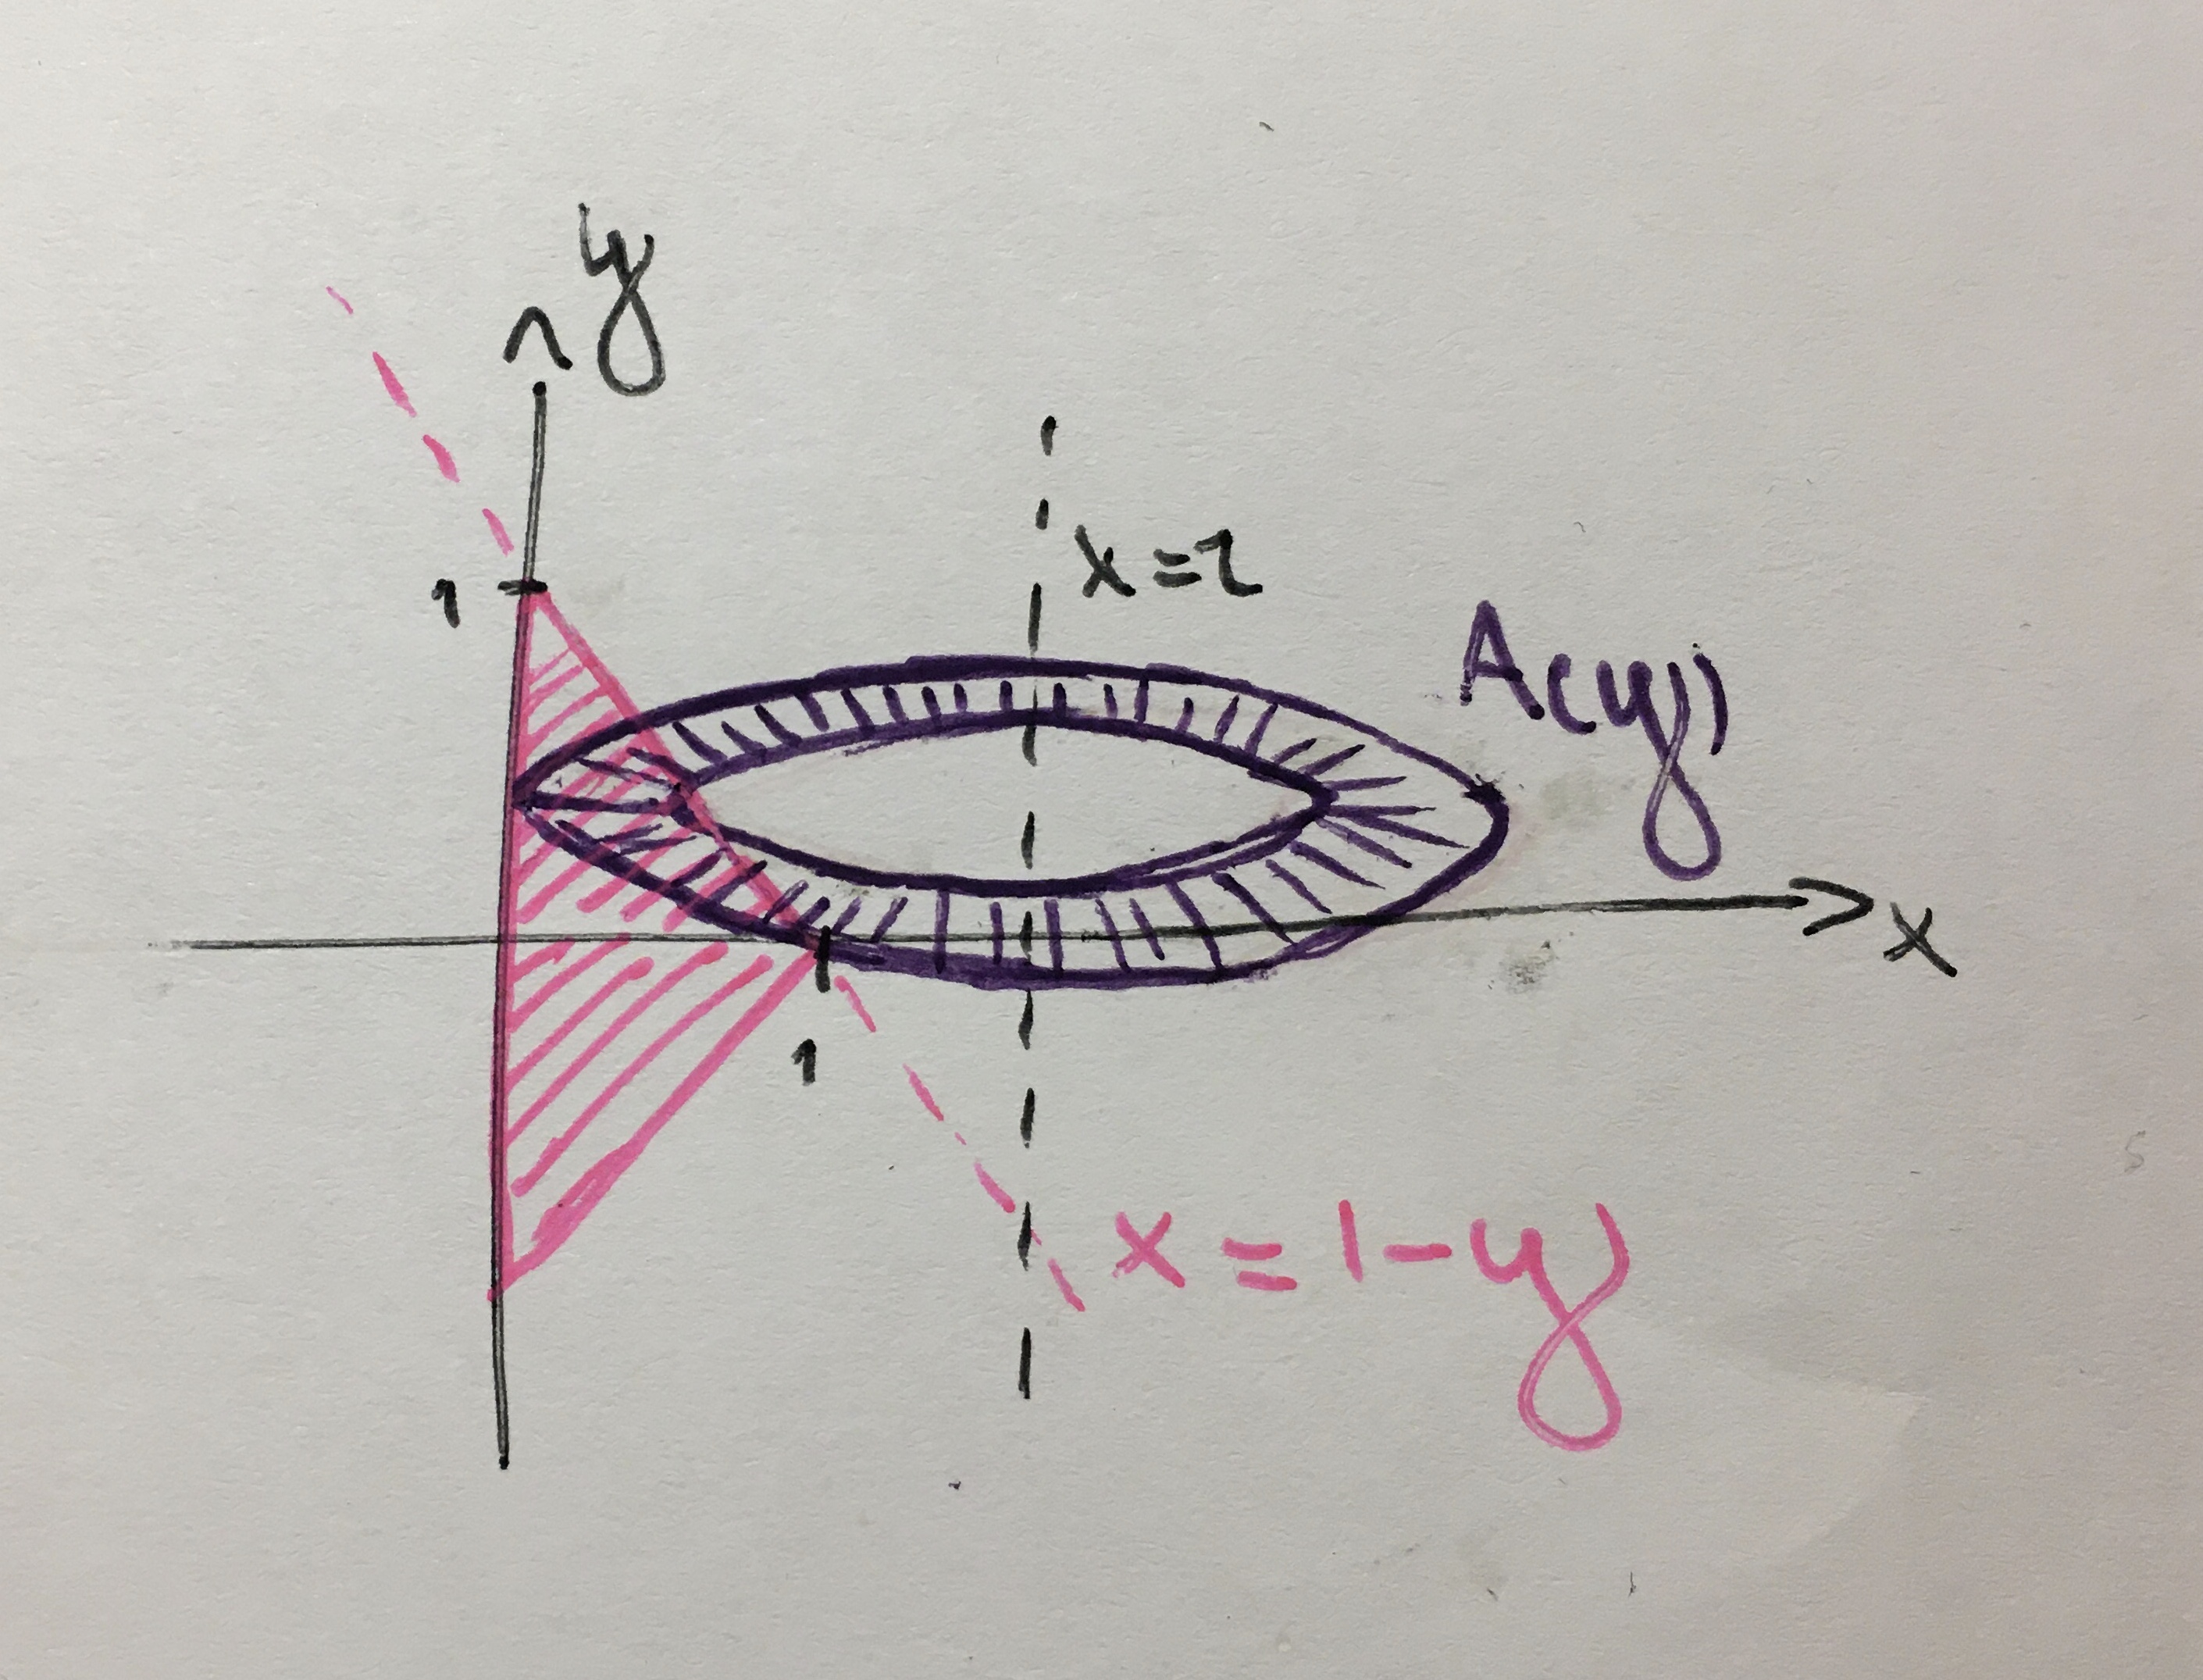
\includegraphics[width=0.6\linewidth]{figures/rotationsvolym_7_1_11.jpg}
	\caption{}%
	\label{fig:figures/rotationsvolym_7_1_11}
\end{figure}

Definera arean $A(y)$ enligt \cref{fig:figures/rotationsvolym_7_1_11}.
Då är
\begin{align*}
	V ={}& 2 \int_0^1 A(y) \dd{y}\\
	={}& 2 \int_0^1 \left(\pi 2^2 - \pi (x - 2)^2\right) \dd{y}\\
	={}& 2 \pi \int_0^1 \left(4 - (-1 - y)^2\right) \dd{y}\\
	={}& \frac{10 \pi}{3}.
\end{align*}


\subsection{7.2 3}%
\label{sub:7_2_3}

Hitta volymen av en figur som har höjd $1$ och vars tvärsnitt vid höjden $z$ är en ellips som har en radie $z$ och en radie $\sqrt{1 - z^2}$.

\paragraph{Lösning:}

Vi gör ungefär som i förra uppgiften.
En ellips med radierna $a$ och $b$ har arean $a b \pi$, så
\begin{align*}
	V ={}& \int_0^1 A(z) \dd{z}\\
	={}& \int_0^1 \pi z \sqrt{1 - z^2} \dd{z}\\
	={}& -\frac{\pi}{3} \int_0^1 \derivative{}{z} \left(1 - z^2\right)^\frac{3}{2} \dd{z}\\
	={}& -\frac{\pi}{3} \left[ \left(1 - z^2\right)^\frac{3}{2} \right]_0^1\\
	={}& \frac{\pi}{3}.
\end{align*}


\subsection{7.2 7}%
\label{sub:7_2_7}

Hitta volymen av en figur som har höjd $h$ och vars tvärsnitt vid höjden $z$ är en cirkelsektor med radien $a$ och vinkel $2 \pi (1 - z / h)$.

\paragraph{Lösning:}

Med $A(z) = \pi a^2 (1 - z / h)$ har vi att

\begin{align*}
	V ={}& \int_0^h A(z) \dd{z}\\
	={}& \int_0^h \pi a^2 (1 - \frac{z}{h}) \dd{z}\\
	={}& \pi a^2 \left[ z - \frac{z^2}{2 h} \right]_0^h\\
	={}& \pi a^2 \frac{h}{2}.
\end{align*}


\subsection{7.9 4}%
\label{sub:7_9_4}

Lös den separabla differentialekvationen
\begin{align*}
	\derivative{y}{x} ={}& x^2 y^2.
\end{align*}

\paragraph{Lösning:}

\begin{align*}
	\derivative{y}{x} ={}& x^2 y^2\\
	\derivative{y}{x} \frac{1}{y^2} ={}& x^2\\
	\derivative{}{x} \left( -\frac{1}{3 y^3} \right) ={}& x^2\\
	-\frac{1}{3 y^3} ={}& \frac{1}{3} x^3 + C\\
	y ={}& -(x^3 + C')^{-1/3}.
\end{align*}
	

\subsection{7.9 12}%
\label{sub:7_9_12}

Lös
\begin{align*}
	\derivative{y}{x} + \frac{y}{x} = \frac{1}{x^2}.
\end{align*}

\paragraph{Lösning:}

\begin{align*}
	\derivative{y}{x} + \frac{y}{x} ={}& \frac{1}{x^2}\\
	x \derivative{y}{x} + y ={}& \frac{1}{x}\\
	\derivative{}{x}{(x y)} ={}& \frac{1}{x}\\
	x y ={}& \log{x}\\
	y ={}& \frac{\log{x}}{x}.
\end{align*}


\subsection{7.9 19}

Lös begynnelsevärdesproblemet
\begin{align*}
	x^2 y' + y ={}& x^2 \exp{1/x},\\
	y(1) ={}& 3 \exp{}.
\end{align*}

\paragraph{Lösning:}

\begin{align*}
	\exp{-1/x} y' + \exp{-1/x} \frac{1}{x^2} y ={}& 1\\
	\derivative{}{x}{(\exp{-1/x} y)} ={}& 1\\
	\exp{-1/x} y ={}& x + C\\
	y ={}& \exp{1/x} (x + C).
\end{align*}
$y(1) = 3 \exp{}$ medför att $C = 2$.


\subsection{Review 7 12}%
\label{sub:review_7_12}

Hitta en familj av kurvor som skär alla ellipser på formen
\begin{align*}
	3 x^2 + 4 y^2 = C
\end{align*}
vinkelrätt.

\paragraph{Lösning:}

I det övre halvplanet kan vi beskriva dessa ellipser som funktioner.
Det gäller då att dessa funktioner uppfyller
\begin{align*}
	6 x + 8 y \derivative{y}{x} ={}& 0\\
	\derivative{y}{x} ={}& -\frac{3 x}{4 y}.
\end{align*}
Men en kurva som är vinkelrät mot denna måste uppfylla (se exempel 6 i avsnitt 7.9 i Adams)
\begin{align*}
	\derivative{y}{x} ={}& \frac{4 y}{3 x}.
\end{align*}
Vi kan lösa denna diffekvation genom variabelseparation, men det går också att se direkt att $y = C x^{4 / 3}$ är en familj lösningar.



